ATLAS utilizes two different calorimeters, the Liquid Argon and Tile Calorimeters~\cite{1996.lar-tdr, 1996.tilecal-tdr}, in order to measure electromagnetic and hadronic objects.
The general principle behind both calorimeters is the same: an incoming particle showers as it passes through and eventually stops, and the resulting energy deposits are read out.
Both are sampling calorimeters, which consist of alternating layers of a dense material to induce the showering (absorber) and a second material which measures the energy (active material).
An advantage to this type of calorimeter is that a very dense absorber can be used in order to produce a shower in a limited space, even if it is unsuitable for measuring the energy from the shower.
However, as some of the energy is deposited in the dense material, and the total shower energy must be estimated.
ATLAS's calorimeter systems are shown in Figure~\ref{fig:calorimeters}.

\begin{figure}[htbp]
  \centering
  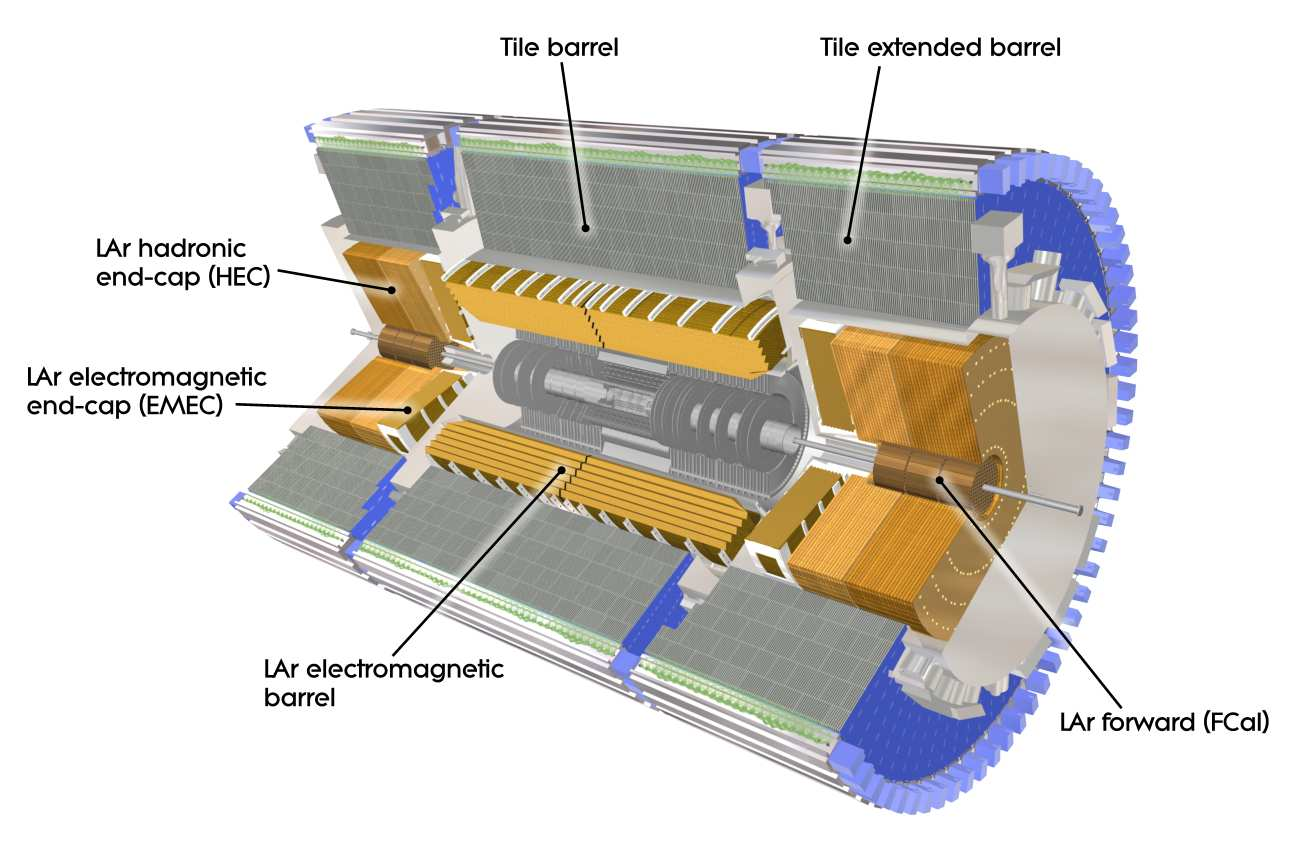
\includegraphics[width=.8\textwidth]{figs/detector/calorimeter}
  \caption[Cut-away view of the ATLAS calorimeter systems.]{Cut-away view of the ATLAS calorimeter systems~\cite{2018.tilecal}.}
  \label{fig:calorimeters}
\end{figure}

Electromagnetic objects, such as electrons and photons, shower via cascades of bremsstrahlung photons and $e^+ e^-$ pairs.
The radiation length $X_0$ is defined as the mean distance over which an electron's energy is reduced to $1/e$ of its original value, or $E(x) = E_{0}e^{-x/X_0}$.
The majority of the shower energy is deposited in the first few radiation lengths.
The longitudinal shower depth scales logarithmically with particle energy, and the transverse shower width is described by the Moli\`{e}re radius\footnote{A cone with a radius equal to the Moli\`{e}re radius ($M_R$) will contain approxiately 90\% of the shower energy.  At a radius of $2M_R$, 95\% of the energy will be contained.} of the material.

Hadronic showers (referred to as \emph{jets}) are the result of quarks or gluons which hadronize and shower primarily via the strong interaction.
Hadronic showers are generally wider than the electromagnetic showers described above.
The longitudinal depth of the hadronic shower scales with the nuclear interaction length of the material $\lambda$, defined as the mean distance for the number of particles in a hadronic jet to be reduced to $1/e$ of the initial number.
In addition, about $1/3$ of the shower products are neutral pions $\pi^0$ which decay electromagnetically.

%Together, the two calorimeters have pseudorapidity coverage up to $|\eta| < 4.9$.

\subsubsection{Liquid Argon Calorimeter} \label{sec:lar}
The LAr Calorimeter contains four individual calorimeters: the electromagnetic barrel (EMB) and endcaps (EMEC), and the hadronic endcap (HEC) and forward calorimeter (FCal).
The calorimeter is surrounded by a cryostat held at a temperature around 90~K.

Focusing on the electromagnetic components first, the EMB covers $|\eta| < 1.475$ and the two EMECs cover $1.375 < |\eta| < 3.2$.
They consist of alternating layers of lead absorber and liquid argon.
The thickness of the lead depends on the location within the detector, but the layers range from 1.1-2.2~mm.
The absorbers are folded into an accordion shape, where the folding angles are varied in order to keep the thickness of the liquid argon gap constant (about 2.1~mm) accross the barrel.
The minimum number of radiation lengths at the end of the electromagnetic calorimeter is $24~X_0$.

There are four layers within the EMB and EMEC including an innermost pre-sampler that helps correct for energy lost before the shower reaches the calorimeter.
The next three layers consist of differently shaped cells successively reducing in granularity.
The first layer consists of narrow strips for fine-grained $\eta$ resolution, and the majority of the shower energy is deposited in the second layer.
The accordion shape as well as the sizes of the cells in the EMB are shown in Figure~\ref{fig:lar_accordion}.

\begin{figure}[htbp]
  \centering
  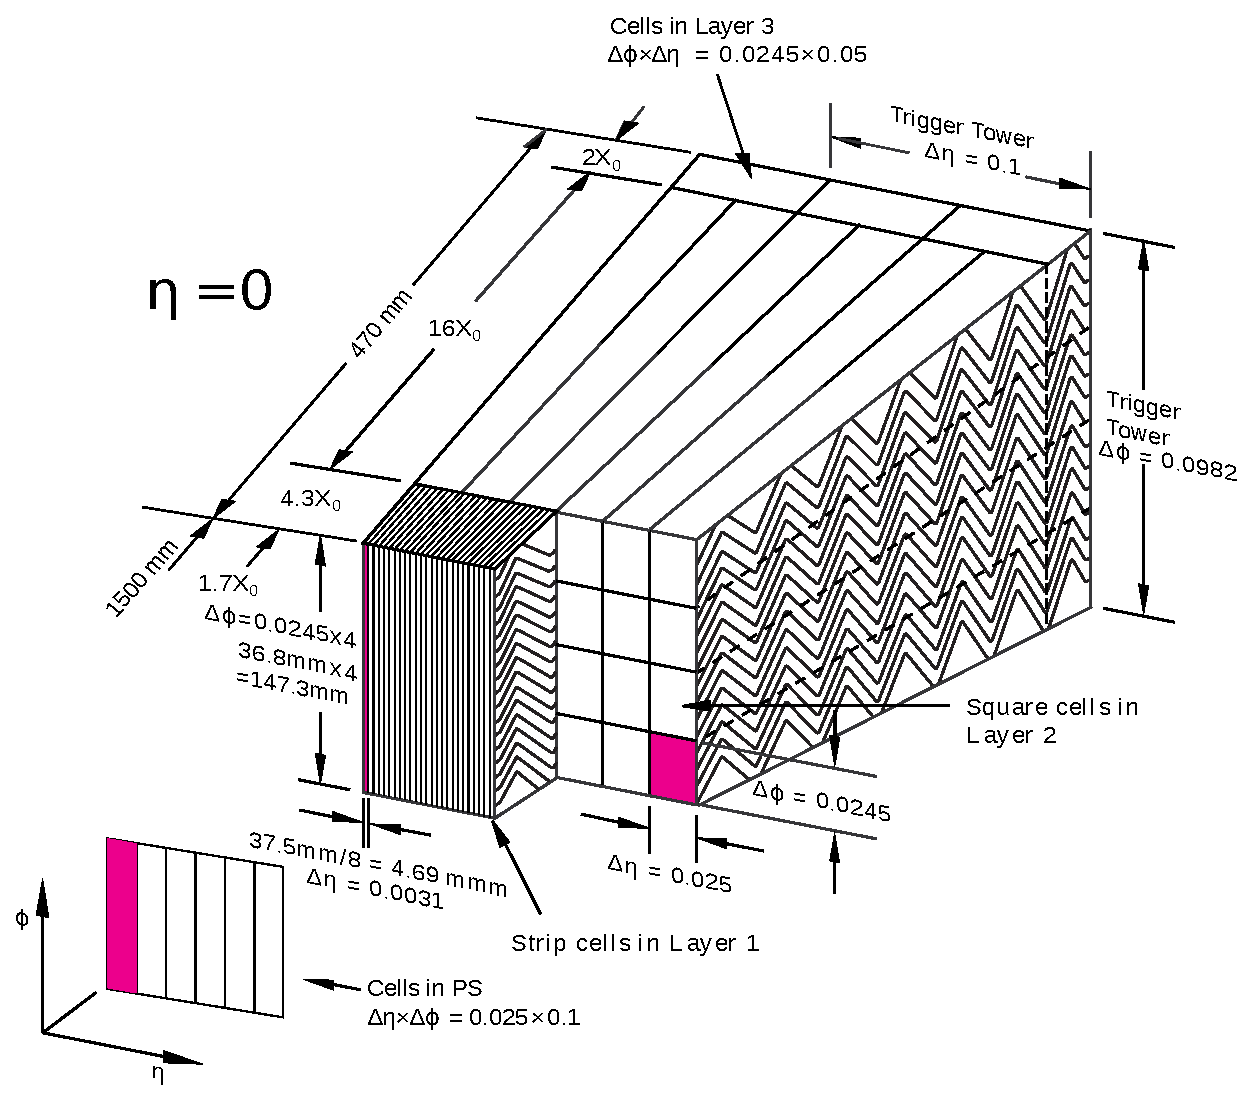
\includegraphics[width=.8\textwidth]{figs/detector/lar_accordion}
  \caption[Diagram of the cells within the LAr barrel.  The accordion structure can be seen in the cut-away view.]{Diagram of the cells within the LAr barrel.  The accordion structure can be seen in the cut-away view~\cite{1996.lar-tdr}.}
  \label{fig:lar_accordion}
\end{figure}

The HEC is located directly behind the EMEC and covers $1.5 < |\eta| < 3.2$.
It uses thick copper plates as the absorber (25~mm in the front wheels and 50~mm in the rear wheels) separated by 8.5~mm gaps filled with liquid argon.
Rather than the accordion shape, the HEC cells are rectangular.

The FCal provides coverage for hadronic jets over the range $3.2 < |\eta| < 4.9$.
Each FCal endcap consists of three layers.
The first is an electromagnetic calorimeter with a copper absorber, while the other two hadronic layers use a tungsten absorber.
Due to the high particle flux entering the FCal, the liquid argon gaps are very narrow, and electrodes are embedded into the absorbers parallel to the beam line.

\subsubsection{Tile Calorimeter}
The TileCal consists of a barrel and two ``extended barrel'' sections which cover the range $|\eta| < 1.7$.
It consists of alternating layers of steel plates and polystyrene scintillator tiles as the absorbers and active material, respectively.
The total thickness of the TileCal is approximately $9~\lambda$.
As the shower passes through the scintillators, photons are emitted that are picked up by wavelength shifting fibers and passed to photomultiplier tubes.
%The resolution of the TileCal is approximately $0.1\times 0.1$ in $\eta$-$\phi$.
